\cleardoublepage
\chapterimage{bg/5}

\chapter{Organisation}


\section{Entreprise}
	J'ai effectué mon stage au sein de l'IRIT --~Institut de Recherche en Informatique de Toulouse, une unité mixte de recherche fondée en 1990 en partenariat entre l'université Paul~Sabatier de Toulouse, le Centre national de la recherche scientifique, l'ENSEEIHT, l'Institut national polytechnique de Toulouse et l’université des Sciences Sociales de Toulouse. L'IRIT comprend 19 équipes de recherche réparties selon sept thèmes~:
	\begin{enumerate}
		\item Analyse et synthèse de l’information~;
		\item Indexation et recherche d’informations~;
		\item Interaction, autonomie, dialogue et coopération~;
		\item Raisonnement et décision~;
		\item Modélisation, algorithmes et calcul haute performance~;
		\item Architecture, systèmes et réseaux~;
		\item Sûreté de développement du logiciel.
	\end{enumerate}
	
	J'ai pour ma part intégré l'équipe SIG\footnote{Systèmes d’Informations Généralisés} dépendant du thème 2 «~Indexation et recherche d’informations~».
	
	La figure~\ref{fig:irit} illustre cette organisation.
	
	\begin{figure}[h]
		\centering
		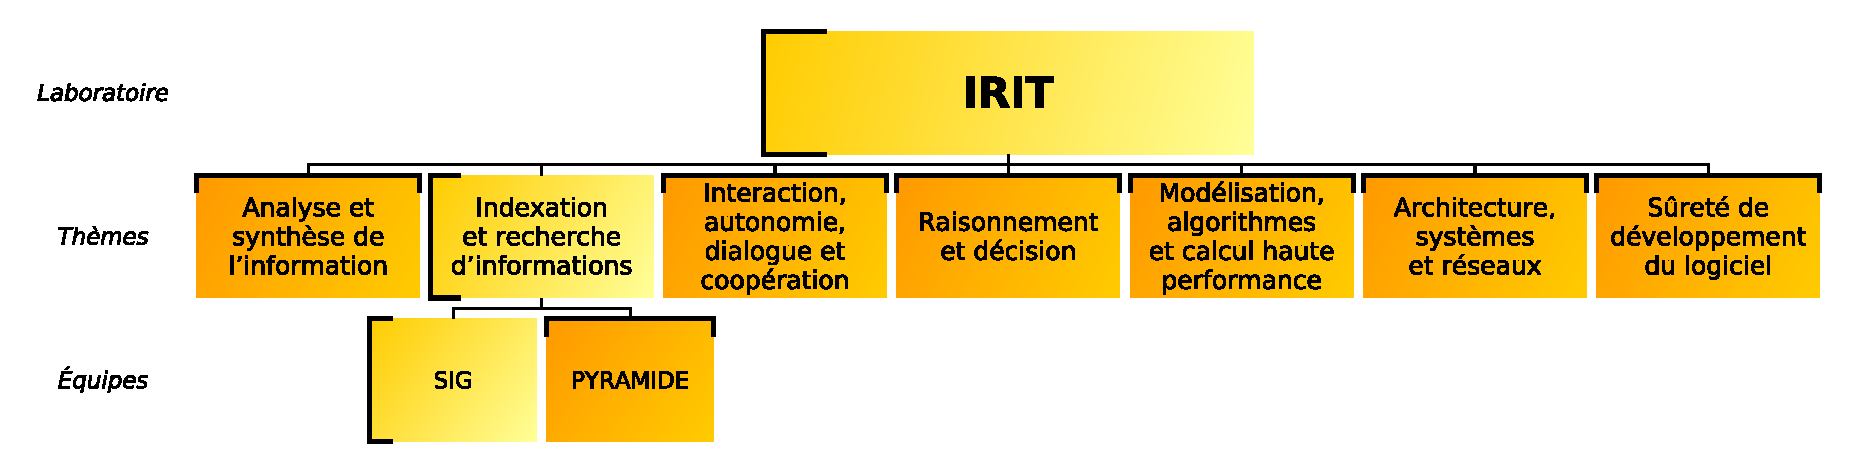
\includegraphics[width=\textwidth]{ch4/irit}
		\caption{Organisation des équipes de recherches de l'IRIT -- il s'agit ici d'une représentation partielle se concentrant sur l'équipe SIG}\label{fig:irit}
	\end{figure}
	
	L'IRIT comprend près de 700 personnes travaillant dans le monde de la recherche, comme illustré sur la figure~\ref{fig:iritDiag}.
	
	\begin{figure}[h]
		\centering
		\begin{subfigure}[b]{0.45\textwidth}
			\centering
			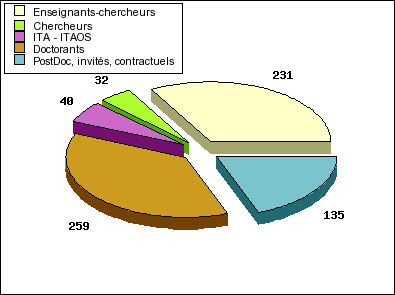
\includegraphics[width=\textwidth]{ch4/iritCat}
			\caption{Par catégorie}
		\end{subfigure}
		\begin{subfigure}[b]{0.45\textwidth}
			\centering
			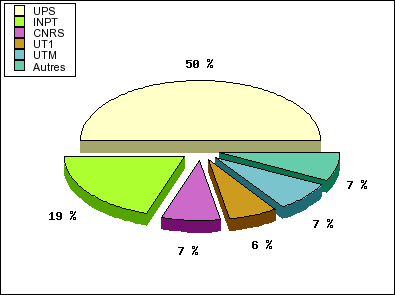
\includegraphics[width=\textwidth]{ch4/iritTutelle}
			\caption{Par tutelle}
		\end{subfigure}
		\caption{Personnel de l'IRIT \citep{irit}}\label{fig:iritDiag}
	\end{figure}


\section{Équipe du projet}
	J'ai travaillé durant ce stage en collaboration avec mon maître de stage, Guillaume~Cabanac. Nous nous sommes basés sur ses précédents travaux en scientométrie.
	
	Guillaume~Cabanac est docteur en informatique et maître de conférences dans l'équipe SIG. Il est enseignant à l'IUT Informatique de Rangueil et à l'université Paul Sabatier. Il est également membre du comité de rédaction des revues scientifiques suivantes qui sont en lien direct avec mon sujet de stage~:
	\begin{itemize}
		\item Scientometrics (depuis 2013),
		\item Roars Transactions (depuis 2013),
		\item Ingénierie des Systèmes d'Information (depuis 2012).
	\end{itemize}
	
	La liste complète de ses publications est disponible sur \href{http://publicationslist.org/guillaume.cabanac}{\texttt{publicationslist.org}}.
	


\section{Planification}

	\subsection{Planning prévisionnel}
		Le diagramme de Gantt prévisionnel de mon stage est représenté sur la figure~\ref{fig:ganttPrev}.
	
		\begin{figure}[p]
			\centering
			\input{tableaux/ch4/gantt}
			\caption{Diagramme de Gantt prévisionnel de mon stage}\label{fig:ganttPrev}
		\end{figure}


	\subsection{Planning effectif}
		Le diagramme de Gantt effectif de mon stage est visible sur la figure~\ref{fig:ganttEff}. On peut constater que ma première mission --~traitant du congrès Inforsid~-- a pris une semaine de plus que le temps estimé. Cependant cela n'a pas eu d'incidence fâcheuse car j'avais surestimé la durée d'autres tâches telles que l'intégration de nouvelles données dans les bases.
		
		Je n'ai pas réalisé l'insertion des comités de rédaction du domaine IA dans la base de travail car je me suis concentrée sur mon étude et n'ai pas trouvé le temps de me concerter avec mon maître de stage sur comment mener à bien cette tâche. Bien que mon planning ait subi quelques ajustements au cours du stage j'ai donc réussi à tenir mes délais et à produire le travail demandé.
	
		\begin{figure}[p]
			\centering
			\input{tableaux/ch4/ganttEff}
			\caption{Diagramme de Gantt effectif de mon stage --~la description des tâches est disponible dans la figure~\ref{fig:ganttPrev}}\label{fig:ganttEff}
		\end{figure}
	